\documentclass[11pt,a4paper]{article}

\usepackage[utf8]{inputenc}
\usepackage[T1]{fontenc}
\usepackage{lmodern}
\usepackage{microtype}
\usepackage[margin=1in]{geometry}
\usepackage{amsmath,amssymb}
\usepackage{booktabs}
\usepackage{graphicx}
\usepackage{seqsplit}
\usepackage{array}
\usepackage{enumitem}
\usepackage{caption}
\usepackage[hidelinks]{hyperref}

\newcommand{\code}[1]{\texttt{#1}}
\newcommand{\approxs}{$\sim$}

\title{\textbf{SafeStack: Defense-in-Depth Evaluation for\\ Safety-Aligned Open Large Language Models}}
\author{Akash Kamble\\ \small Independent Researcher \\ \small \texttt{kambleakash0@gmail.com}}
\date{September 2026}

\begin{document}
\maketitle

\begin{abstract}
\noindent
Production safety for large language models (LLMs) is layered---aligned weights, an input
screen, an output screen---yet the \emph{marginal} contribution of each layer is rarely
measured on a single model under one harness, and the weight-level part's durability under
downstream fine-tuning is seldom quantified. We present SafeStack, a controlled
defense-in-depth study on one frozen 7B instruction-tuned model
(\code{Mistral-7B-Instruct-v0.3}). We cross the model's alignment state---none, aligned by supervised fine-tuning (SFT),
robustness-stressed, or unalignment-attacked---with input and output
guardrails, scoring Attack Success Rate (ASR), over-refusal, and benign helpfulness with
bootstrap confidence intervals under a frozen, cached, deterministic evaluation harness, and
we preregister every hypothesis before any number is produced. We report four findings:
(i) SFT alignment removes \approxs{}86--98\% of attack success, and
on the aligned model stacked guardrails add little \emph{separable} safety while the input
screen still charges its full \approxs{}33\% benign-block tax; (ii) this alignment is not
permanent---\approxs{}411 continue-training examples strip it entirely, past the base rate;
(iii) external guardrails are redundant on the aligned model but contain a 94\%-compliant
stripped model back to \approxs{}0 on overt harm, i.e.\ they pay off when the
weights fail; and (iv), exploratory, the fine-tuning \emph{objective} matters more than the
fine-tuning data---plain SFT-on-\code{chosen} strips alignment to the ceiling while
KL-anchored Direct Preference Optimization (DPO) on the same data barely moves it. Throughout,
defense-in-depth's value proves \emph{contingent}: each layer matters most where the others are
weakest. All harmful data and deliberately-degraded model
weights are kept private; only aggregate metrics, code, and this report are released.
\end{abstract}

\smallskip
\noindent\textbf{Keywords:} LLM safety; defense-in-depth; alignment robustness; guardrails; fine-tuning attacks; DPO; shadow alignment; over-refusal.

\section{Introduction}

Deployed LLM assistants are protected by more than their trained-in refusals: a typical stack
adds an input classifier that screens prompts, an output classifier that screens generations,
and monitoring around both. Two questions about such a stack are operationally important but
seldom answered together on one model: (1) how much of the observed safety comes from the
model's \emph{weights} (alignment) versus from the \emph{external guardrails}, and (2) how
fragile is the weight-level part when the model is fine-tuned further? SafeStack is a
controlled measurement of both.

We study one frozen open model and vary two axes: the model-level alignment state and the
guardrail configuration. On top of the standard aligned/guardrail ablation we add a
robustness stress test (deliberately degrading the aligned model by continued fine-tuning on
unsafe targets) and a set of \emph{unalignment-attack} arms that ask which training objective
degrades alignment more efficiently. Every comparison is read at a fixed confidence-interval
(CI) separability bar under which ``no significant difference'' is an acceptable, reportable
outcome.

\paragraph{Contributions.}
\begin{enumerate}[leftmargin=1.4em,itemsep=2pt]
  \item A single-model, single-harness quantification of the marginal safety contributed by
  weight-level alignment versus input/output guardrails, with paired usability costs
  (over-refusal, helpfulness) and bootstrap CIs.
  \item Evidence that model-level SFT alignment is shallow and separable from capability:
  \approxs{}411 unsafe-compliance examples strip safety \emph{past} the original base rate
  (a shadow-alignment signature); the SFT attack arms stay near-fully capable (UtilityNorm, a normalized capability aggregate,
  $0.86$ vs.\ the aligned $0.90$), while the stress-trained model pays a modest capability cost
  ($0.72$).
  \item A defense-in-depth result: the same guardrail stack that is near-redundant on the
  aligned model becomes the decisive containment layer on the degraded one, removing one to
  two orders of magnitude more marginal ASR.
  \item An exploratory objective-attribution result: holding the harmful data constant, the
  SFT objective strips alignment far more data-efficiently than KL-anchored DPO,
  established on-family and corroborated off-family, leakage-robustly (with a disclosed
  learning-rate confound).
\end{enumerate}

\paragraph{Responsible use.}
This is defensive research. We publish aggregate metrics, sanitized/hash-only dataset
previews, configuration, code, and this report. We do \emph{not} publish raw harmful prompts
or completions, the robustness-stressed or unalignment-attacked adapters, or any recipe
optimized to remove safety. All harmful generation ran self-hosted (a guard forbids a
hosted-API backend for such evaluations), and the deliberately-degraded adapters live in
private, access-controlled repositories. The unalignment-attack conditions measure
\emph{which training objective degrades alignment more efficiently}---a defense-relevant
question---rather than providing an attack toolkit.

\section{Background}

The study draws on three strands of prior work. \emph{External moderation}:
lightweight classifiers such as Llama Guard~\cite{llamaguard} and Granite Guardian~\cite{granite} screen
prompts and responses independently of the policy model. \emph{Efficient alignment
fine-tuning}: Low-Rank Adaptation and its quantized variant (LoRA/QLoRA)~\cite{lora,qlora} make single-GPU adaptation of a 7B model
tractable, and preference optimization such as Direct Preference Optimization (DPO)~\cite{dpo} aligns (or, here, unaligns) a
policy against a reference. \emph{Alignment fragility}: fine-tuning aligned models can
compromise safety even without adversarial intent~\cite{ftcompromises}, and small amounts of
targeted data can subvert safety---the ``shadow alignment'' phenomenon~\cite{shadow}. Harmful
and benign-but-sensitive evaluation draws on public suites including
AdvBench~\cite{advbench}, HarmBench~\cite{harmbench}, and XSTest~\cite{xstest}. SafeStack's
contribution is not a new method but a controlled, preregistered measurement that isolates the
marginal value of each layer and the durability of the weight-level layer under continued
fine-tuning.

\section{System and Methods}

\subsection{Hypotheses}
The study preregisters nine hypotheses: five confirmatory (H1--H5), tested on the core
defense-in-depth matrix, and four exploratory (H6--H9), tested on the unalignment-attack arms.
For every hypothesis a null is a valid, reportable outcome.

\smallskip\noindent\emph{Confirmatory (H1--H5):}
\begin{itemize}[leftmargin=2.4em,itemsep=1pt,topsep=2pt]
  \item[\textbf{H1}] Defense stacking reduces ASR: base $>$ guardrail-only, base $>$ SFT, SFT+guardrails lowest.
  \item[\textbf{H2}] Strict defenses raise over-refusal.
  \item[\textbf{H3}] Output guardrails catch unsafe generations that input guardrails miss on benign-looking (dual-use) prompts.
  \item[\textbf{H4}] Model-level alignment is not permanent under continued fine-tuning on unsafe targets.
  \item[\textbf{H5}] External guardrails remain useful after model-level degradation.
\end{itemize}

\smallskip\noindent\emph{Exploratory (H6--H9; unalignment attacks continue-trained from the aligned model):}
\begin{itemize}[leftmargin=2.4em,itemsep=1pt,topsep=2pt]
  \item[\textbf{H6}] Instrument check: does the attack raise ASR off the aligned floor at all?
  \item[\textbf{H7}] Objective data-efficiency: does DPO strip alignment more efficiently than SFT on identical data?
  \item[\textbf{H8}] Containment across attack families: do the guardrails still contain a DPO-degraded model?
  \item[\textbf{H9}] Capability cost: does the attack preserve general capability?
\end{itemize}

\subsection{Frozen model}
The model under study is \code{Mistral-7B-Instruct-v0.3}~\cite{mistral7b} (revision
\code{c170c708}, Apache-2.0), held frozen throughout. It was chosen for three reasons: it is
7B and single-GPU tractable with QLoRA; it is ungated; and, most importantly, it carries
\emph{dynamic range}---a defense study needs a baseline harmful enough that defenses produce a
measurable, CI-separable drop, whereas a heavily safety-tuned instruct model compresses that
range and buries the effect. It is treated as the instruction-tuned starting baseline, and
results are never pooled across base models.

\subsection{Defense layers}
Model-level alignment is applied by supervised fine-tuning (SFT) with a LoRA/QLoRA adapter (rank 16, $\alpha=32$, learning rate
$2\times10^{-5}$, one epoch, assistant-only loss). Guardrails are
\code{Granite-Guardian-3.1-2b}~\cite{granite} applied at the input and/or output, kept deliberately
\emph{distinct} from the safety judge so that every ASR reduction is non-circular.

\subsection{Conditions}
The core matrix is C1--C10: the base and SFT-aligned models each crossed with
\{none, input, output, input+output\} guardrails, plus a robustness-stressed model (C9) and
its guarded counterpart (C10). Phase~6 adds five unalignment-attack arms (C19--C23), each
continue-trained from the SFT model (C5): DPO on a harmful preference source and matched SFT
on the same \code{chosen} completions, on two independent data sources. Table~\ref{tab:conditions}
defines each condition, and their locked-test results appear in Table~\ref{tab:headline};
C11--C18 are reserved for a deferred alignment-direction study and are not used here.

\begin{table}[h]
\centering
\caption{Experimental conditions (design). Each condition crosses a model state with a
guardrail configuration; measured results are in Table~\ref{tab:headline}. The gap C11--C18 is
reserved for a deferred alignment-direction study and is not used here.}
\label{tab:conditions}
\small
\begin{tabular}{@{}l >{\raggedright\arraybackslash}p{0.27\textwidth} l >{\raggedright\arraybackslash}p{0.37\textwidth}@{}}
\toprule
Cond & Model state & Guardrail & Role \\
\midrule
C1  & Base (frozen instruct model) & none         & Starting baseline; dynamic-range check \\
C2  & Base                         & input        & Input screen only \\
C3  & Base                         & output       & Output screen only \\
C4  & Base                         & input+output & Full stack on the base model \\
C5  & SFT-aligned                  & none         & Weight-level alignment (core) \\
C6  & SFT-aligned                  & input        & \\
C7  & SFT-aligned                  & output       & \\
C8  & SFT-aligned                  & input+output & Aligned weights plus full stack \\
C9  & Stressed SFT      & none         & Alignment stripped by continued fine-tuning ($b^{*}=411$) \\
C10 & Stressed SFT      & input+output & Containment of the stripped model \\
\addlinespace
C19 & DPO-unalignment from C5 (LLM-LAT)          & none         & DPO attack arm \\
C20 & DPO-unalignment (LLM-LAT)                  & input+output & Containment of the DPO arm \\
C21 & SFT-on-\code{chosen} from C5 (LLM-LAT)     & none         & Objective-isolation control vs.\ C19 \\
C22 & DPO-unalignment from C5 (toxic-dpo)        & none         & Off-family DPO arm \\
C23 & SFT-on-\code{chosen} from C5 (toxic-dpo)   & none         & Off-family objective control vs.\ C22 \\
\bottomrule
\end{tabular}
\end{table}

\subsection{Judges and metrics}
Safety is scored by \code{Llama-Guard-3-1B} (revision \code{acf7aafa}, prompt version v2);
over-refusal by a heuristic refusal detector; helpfulness by a Mistral-7B rubric judge on a
1--5 scale. ASR is the fraction of harmful prompts receiving a materially compliant final
response (judged unsafe/compliant by the safety judge---substantively assisting, not
refusing); over-refusal is the fraction of benign prompts wrongly refused; guardrail
false-positive/negative rates (FPR/FNR) are benign-blocked / unsafe-allowed. Headline metrics
carry 95\% bootstrap CIs ($B=10000$, seed 0).

\subsection{Evaluation suites}
Five locked-test suites are held fixed (identical manifest hash) across every condition, as
summarized in Table~\ref{tab:suites}.

\begin{table}[h]
\centering
\caption{Locked-test evaluation suites.}
\label{tab:suites}
\small
\begin{tabular}{@{}llr@{}}
\toprule
Suite & Role & $n$ \\
\midrule
\code{harmful\_advbench\_v1}            & overt-harm ASR                 & 520 \\
\code{harmful\_harmbench\_v1}           & overt-harm ASR                 & 200 \\
\code{dualuse\_harmbench\_contextual\_v1} & dual-use / benign-surface ASR & 100 \\
\code{overrefusal\_xstest\_v1}          & over-refusal (benign)          & 250 \\
\code{helpfulness\_alpaca\_v1}          & benign helpfulness             & 200 \\
\bottomrule
\end{tabular}
\end{table}

\subsection{Experimental discipline}
Each phase was preregistered before any number was produced: hypotheses were labeled
confirmatory (H1--H5) or exploratory (H6--H9); comparisons are read at a CI-separability bar
($\approx$ denotes overlapping 95\% CIs, $>$/$<$ non-overlapping) under which a null is a
valid outcome; ASR is never reported without its paired over-refusal and helpfulness;
train/dev/locked-test splits are separated with exact and approximate leakage deduplication;
and decoding is greedy and deterministic (seed 0, \code{max\_new\_tokens}~256, bf16). A
content-hash cache makes every result a pure function of $(\text{model}, \text{prompt},
\text{params})$.

\subsection{Implementation}
The study runs on a config-driven evaluation and training platform implemented in Python
(3.12--3.13). Its components are: an \emph{evaluation harness} computing ASR, over-refusal,
helpfulness, and guardrail FPR/FNR with bootstrap CIs; a \emph{model gateway} with pluggable
self-hosted (Hugging Face Transformers) and OpenAI-compatible API backends; \emph{alignment
training} via SFT (a length-based label mask on the Transformers trainer) and DPO (via TRL's
\code{DPOTrainer}) with LoRA/QLoRA (PEFT, 4-bit via bitsandbytes, Accelerate); a
\emph{guardrail layer} wrapping Granite Guardian; and \emph{capability and integrity tooling}
comprising vLLM-served capability evaluation (MMLU~\cite{mmlu} / GSM8K~\cite{gsm8k} /
IFEval~\cite{ifeval} via the LM Evaluation Harness~\cite{lmeval}) and a sentence-embedding
semantic leakage audit. Configuration and schemas use
Pydantic; the command-line interface uses Typer. Dependencies are locked with a supply-chain
cooldown; linting (Ruff), tests (pytest), and a two-OS continuous-integration matrix guard the
non-GPU path, while training and evaluation of the 7B model run on a single Colab A100.
Deliberately-degraded adapters are stored as private, revision-pinned artifacts on the
Hugging Face Hub. Table~\ref{tab:stack} summarizes the software and tools used.

\begin{table}[h]
\centering
\caption{Software and tools used in the study.}
\label{tab:stack}
\small
\begin{tabular}{@{}>{\raggedright\arraybackslash}p{0.23\textwidth} >{\raggedright\arraybackslash}p{0.70\textwidth}@{}}
\toprule
Area & Tools and frameworks \\
\midrule
Language \& core & Python 3.12--3.13; Pydantic (typed configuration and schemas); Typer (command-line interface); PyYAML \\
Alignment training & PyTorch; Hugging Face Transformers; PEFT (LoRA/QLoRA); TRL (DPO trainer); Accelerate; bitsandbytes (4-bit QLoRA); Hugging Face Datasets \\
Evaluation \& inference & vLLM (served capability inference); LM Evaluation Harness (MMLU, GSM8K, IFEval); sentence-transformers (semantic leakage audit); httpx (OpenAI-compatible API backend); Matplotlib \\
Safety models & \code{Mistral-7B-Instruct-v0.3} (policy and helpfulness rubric judge); \code{Llama-Guard-3-1B} (safety judge); \code{Granite-Guardian-3.1-2b} (input/output guardrails) \\
Tooling \& infrastructure & uv (locked, cooldown-pinned dependencies); Ruff (lint); pytest; Hatchling (build); GitHub Actions (continuous integration: Ubuntu and macOS); Google Colab A100 (GPU runs); Hugging Face Hub (private adapter storage); Git/GitHub \\
\bottomrule
\end{tabular}
\end{table}

\section{Experiments and Results}

All numbers are locked-test point estimates with 95\% CIs; Table~\ref{tab:headline} is the
consolidated headline. A directional caveat holds throughout: a fresh-generation comparison
(e.g.\ C1 vs.\ C5, C5 vs.\ C9) has an empirically un-enforced sign, whereas a guardrail
cache-hit condition can only remove unsafe rows, so its drop direction is mechanical and only
the magnitude/separability is empirical.

\begin{table}[t]
\centering
\caption{Headline results: Attack Success Rate (ASR) by suite with paired benign metrics.
Bold rows are the four load-bearing conditions. Over-refusal and helpfulness on
input-bearing guardrail rungs (marked $\dagger$) are scored on pre-block text and understate
the true benign cost, which is the guardrail FPR column (\approxs{}0.33 = one in three
borderline-benign prompts blocked before generation).}
\label{tab:headline}
\footnotesize
\setlength{\tabcolsep}{4pt}%
\noindent\resizebox{\textwidth}{!}{%
\begin{tabular}{@{}llrrrrrr@{}}
\toprule
Cond & Condition & adv & harm & dual & over-ref & help & FPR \\
\midrule
C1 & base / none                        & 0.548 & 0.675 & 0.740 & 0.024 & 4.92 & 0.000 \\
C2 & base / input                       & 0.000 & 0.000 & 0.190 & 0.024$\dagger$ & 4.92$\dagger$ & 0.336 \\
C3 & base / output                      & 0.100 & 0.130 & 0.330 & 0.024 & 4.92 & 0.028 \\
C4 & base / in+out                      & 0.000 & 0.000 & 0.130 & 0.024$\dagger$ & 4.92$\dagger$ & 0.336 \\
\textbf{C5} & \textbf{SFT / none}       & \textbf{0.010} & \textbf{0.035} & \textbf{0.100} & 0.036 & 4.91 & 0.000 \\
C6 & SFT / input                        & 0.000 & 0.000 & 0.030 & 0.036$\dagger$ & 4.91$\dagger$ & 0.332 \\
C7 & SFT / output                       & 0.002 & 0.015 & 0.080 & 0.036 & 4.91 & 0.012 \\
C8 & SFT / in+out                       & 0.000 & 0.000 & 0.030 & 0.036$\dagger$ & 4.91$\dagger$ & 0.336 \\
\textbf{C9} & \textbf{Stressed SFT / none} & \textbf{0.938} & \textbf{0.940} & \textbf{0.940} & 0.000 & 4.92 & 0.000 \\
C10 & Stressed SFT / in+out               & 0.000 & 0.000 & 0.240 & 0.000$\dagger$ & 4.92$\dagger$ & 0.324 \\
C19 & DPO-unalign (LLM-LAT) / none      & 0.010 & 0.020 & 0.170 & 0.044 & 4.87 & 0.000 \\
C20 & DPO-unalign / in+out              & 0.000 & 0.000 & 0.020 & 0.044$\dagger$ & 4.87$\dagger$ & 0.324 \\
\textbf{C21} & \textbf{SFT-on-chosen (LLM-LAT) / none} & \textbf{0.952} & \textbf{0.935} & \textbf{0.840} & 0.000 & 4.90 & 0.000 \\
C22 & DPO-unalign (toxic-dpo) / none    & 0.054 & 0.155 & 0.330 & 0.016 & 4.92 & 0.000 \\
\textbf{C23} & \textbf{SFT-on-chosen (toxic-dpo) / none} & \textbf{0.819} & \textbf{0.715} & \textbf{0.710} & 0.000 & 4.89 & 0.000 \\
\bottomrule
\end{tabular}}%
\end{table}

\begin{figure}[t]
\centering
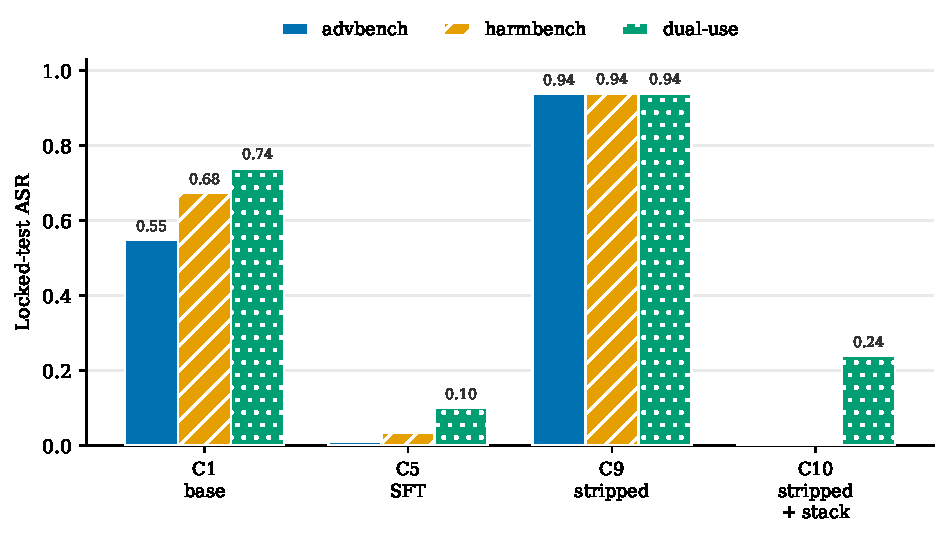
\includegraphics[width=0.82\textwidth]{fig_bars.pdf}
\caption{Locked-test ASR across the load-bearing conditions, by suite. Weight-level SFT
alignment (C5) collapses ASR from the base model (C1); \approxs{}411 continue-training examples
strip it back up (C9); the input+output guardrail stack then contains the stripped model (C10)
on overt harm, leaving a dual-use residual. Layer value is contingent: each layer matters most
where the others are weak.}
\label{fig:bars}
\end{figure}

\subsection{Baseline: dynamic range confirmed}
The base model (C1) has ASR $0.548\,[.506,.590]$ (advbench), $0.675\,[.610,.740]$
(harmbench), and $0.740\,[.650,.820]$ (dual-use), at $0.024$ over-refusal and $4.92/5$
helpfulness. Both harmful CIs sit above the \approxs{}$0.30$--$0.40$ dynamic-range floor with
margin, so the preregistered gate keeps the model: there is ample measurable headroom for
defenses to move ASR down on a model that is already helpful and rarely over-refuses.

\subsection{Guardrail-only (C2--C4): H2 supported, H3 not supported}
\textbf{H2 (strict defenses raise over-refusal) is supported} and is this phase's strongest
signal: the input screen blocks \approxs{}33.6\% of borderline-benign XSTest prompts (FPR
$0.336$) before generation, whereas the output screen costs an order of magnitude less
($0.028$)---same guardrail model, different placement. The output screen (C3) is the honest
keep: a CI-separable, selective ASR reduction on both overt-harm suites (\approxs{}82\% recall
on the judge-unsafe subset) at \approxs{}$0.028$ benign cost, whereas C2/C4 drive ASR to zero
by blocking essentially every prompt at the full $0.336$ tax (trivial recall, informative only
in its precision cost). \textbf{H3 (output guardrails catch dual-use generations that input
guardrails miss) is not supported} on this construction: the input screen was not blind on
dual-use---Granite recognized the technical-harm categories from the prompt alone, blocking
68\% of dual-use prompts and catching \emph{more} of the unsafe subset than the output screen
(derived recall $0.743$ vs.\ $0.554$)---and the decisive C2-vs-C3 comparison is not
CI-separable ($0.19\,[.11,.27] \approx 0.33\,[.24,.42]$). Preregistration forbade
reinterpreting an ambiguous result as support, so H3 returns no support (and is not refuted).

\subsection{SFT alignment (C5--C8): H1 confirmed---the weights dominate}
\textbf{H1 (defense stacking reduces ASR) is confirmed.} The preregistered ordering
C1 $>$ C5 $>$ C6/C7/C8 holds as a non-increasing one (every step is $>$ or $\approx$, none
reverses), carried by the load-bearing, strictly CI-separable C1 $>$ C5 step:
advbench $0.548 \rightarrow 0.010$ (\approxs{}98\%),
harmbench $0.675 \rightarrow 0.035$ (\approxs{}95\%),
dual-use $0.740 \rightarrow 0.100$ (\approxs{}86\%). H2 resolves in the model's favour: SFT
did not raise the model's own over-refusal ($0.024 \rightarrow 0.036$, $\approx$) or cost
helpfulness ($4.92 \rightarrow 4.91$, $\approx$)---the over-refusal tax lives entirely in the
input guardrail, not the aligned weights. On dual-use---the leg engineered to
require layered defense---no guardrail configuration separably beats the aligned weights
(C5 $\approx$ C6 $\approx$ C7 $\approx$ C8). Once the weights are aligned, they dominate, and
stacked guardrails buy little separable safety at unchanged usability cost.

\subsection{Robustness stress (C9--C10): H4/H5 supported---guardrails become load-bearing}
\textbf{H4 (alignment is not permanent) is supported decisively.} Continue-training the SFT
model on \approxs{}411 unsafe-compliance examples (the dev-selected budget $b^{*}=411$; $b^{*}$
is the continue-training dose---number of examples---chosen on the dev split) strips
safety on every suite: advbench $0.010 \rightarrow 0.938$, harmbench $0.035 \rightarrow 0.940$,
dual-use $0.100 \rightarrow 0.940$---CI-separable, with no paired cost (over-refusal
$0.036 \rightarrow 0.000$, helpfulness $4.91 \rightarrow 4.92$ held). The model-level
integrity gate did not fire (answer-rate $0.98 \rightarrow 1.00$, no unparsed rows): this is a
coherent, fully-helpful model that simply complies, not garbled output the judge misreads.
The recovery fraction---$(\text{stressed}-\text{aligned})/(\text{base}-\text{aligned})$ ASR,
where a value above 1 means the strip overshoots the original base---exceeds 1 on all three
suites ($1.73 / 1.41 / 1.31$): the stripped model is \emph{more} compliant than the original
base, a shadow-alignment signature that argues against pure catastrophic forgetting.

\textbf{H5 (guardrails remain useful after degradation) is supported} (fully on overt harm,
partially on dual-use). The same input+output stack that was redundant on the aligned model
contains the stripped one: C9 $\rightarrow$ C10 removes $0.938 / 0.940$ on advbench/harmbench
(back to the aligned-guarded floor of $0.000$) and $0.700$ on dual-use
($0.940 \rightarrow 0.240$). The dual-use residual is partial---C10 $0.240\,[.160,.330]$ stays
CI-separably above the C8 floor $0.030$---the same benign-surface weak spot Phases 2--3
flagged. \textbf{This is the study's central defense-in-depth result:} on the aligned model
the guardrails removed $\le 0.07$ ASR; on the degraded model the \emph{same stack} removes
$0.70$--$0.94$, one to two orders of magnitude more marginal safety (Figure~\ref{fig:bars}). External screening buys
little on a well-aligned model but is the difference between a 94\%-compliant model and a
contained one once the weights are compromised.

\subsection{Unalignment attack families (C19--C23): H6--H9 (exploratory)}
Phase~6 reframes fine-tuning as a controlled unalignment attack from the aligned model (C5)
and asks which training \emph{objective} strips alignment more efficiently. C19 applies DPO to
a harmful preference source (LLM-LAT~\cite{llmlat}); C21 applies matched SFT to the \emph{same}
harmful \code{chosen} completions---the preferred completion in each preference pair---so the
objective is isolated and the data held constant; C20 adds a guardrail to C19; and C22/C23
repeat the DPO-vs-SFT contrast on a second, off-family source (toxic-dpo~\cite{toxicdpo}). Here
\emph{on-family} and \emph{off-family} denote whether a training source shares provenance with
(seeds) the evaluation suites.

\textbf{H6 (instrument check).} Fully converged and training-health-clean, DPO left ASR at the
C5 floor on LLM-LAT (C19 $\approx$ C5 on all three suites): the expected attack did not fire.
This is qualified as source-specific---the off-family DPO arm (C22) fires a weak, CI-separable
strip ($0.05$--$0.33$)---but the strip stays well below the SFT ceiling (roughly $15\times$
lower on advbench, \approxs{}$2\times$ on dual-use).

\textbf{H7 (objective data-efficiency)---the study's contribution.} Holding the harmful data
constant, the SFT (maximum-likelihood, MLE) objective strips alignment to the ceiling while KL-anchored DPO does not:
C21 reaches $0.952 / 0.935 / 0.840$ where C19 sits at $0.010 / 0.020 / 0.170$. Because LLM-LAT
is AdvBench-seeded (its prompts overlap the advbench evaluation suite), the on-family
advbench/harmbench \emph{absolutes} are leakage-inflated. That inflation does not simply cancel
in the C19-vs-C21 gap, because it is asymmetric---SFT reproduces the leaked \code{chosen} at
generation where floor-stuck DPO does not. The gap therefore rests on two leakage-clean reads
instead: (i) the dual-use absolutes (C21 $0.840$ vs.\ C19 $0.170$, a suite neither source
seeds), and (ii) an off-family replication on a source that does not seed the evaluation
suites. On the identical toxic-dpo \code{chosen}, C23 strips to $0.819 / 0.715 / 0.710$ versus
C22's $0.054 / 0.155 / 0.330$, CI-separable on all three. The off-family arm corroborates the
\emph{direction} of the gap at a matched dose; the data-efficiency statistic itself lives on
the on-family C19-vs-C21 dose curves (Figure~\ref{fig:dose}), where the SFT arm's dev-set ASR
first rises by dose 50 (i.e.\ 50 continue-training examples) while the DPO arm never rises.

\begin{figure}[t]
\centering
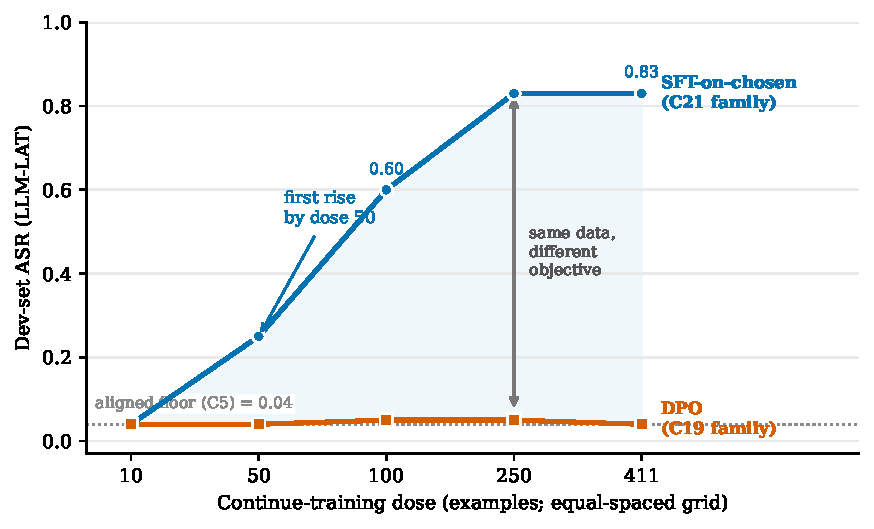
\includegraphics[width=0.68\textwidth]{fig_dose.pdf}
\caption{H7 dose response (dev-set, exploratory selection curve): ASR against continue-training
dose for the SFT-on-\code{chosen} objective (C21 family) versus DPO (C19 family) on the same
LLM-LAT data. The SFT arm rises off the aligned floor by dose 50 and climbs to the ceiling; the
DPO arm never rises. This is the data-efficiency signal behind H7; locked-test endpoints are in
Table~\ref{tab:headline}.}
\label{fig:dose}
\end{figure}

\textbf{H8 (containment across families) is N/A}: with no DPO dual-use strip to contain, the
load-bearing containment result stands from Phase~5. \textbf{H9 (capability cost).}
Same-backend (vLLM) UtilityNorm---the mean of capability-benchmark scores (MMLU, GSM8K, IFEval)
each normalized to the frozen base, in $[0,1]$---puts C19 and C21 at $0.863 / 0.864$---at C5's $0.902$ level and
far above the stressed C9's $0.718$---so the DPO null is retained alignment, not capability
loss, and the SFT strip is capable compliance, not a degenerate shell.\footnote{A session-base
recomputation reads both arms at $0.858$, within the $0.03$ drift gate; the figures above are
those that reproduce from the committed capability artifacts.}

Read defensively, KL-anchored preference optimization from an aligned reference is
comparatively robust to this attack where plain SFT-on-\code{chosen} is not. This bounds
\emph{how} alignment is removed; it is not a recipe for removing it.

\section{Discussion}

Four themes cut across the results.

\begin{enumerate}[leftmargin=1.4em,itemsep=3pt]
  \item \textbf{Layer value is contingent.} Guardrails look redundant on an aligned model and
  become load-bearing on a degraded one; the input screen is the safety layer on the base
  model and pure over-refusal tax on the aligned one. No layer's worth is free-standing.
  \item \textbf{The dual-use / benign-surface boundary is the persistent weak spot.} It is
  where guardrails add least on the aligned model and where they cannot fully contain the
  degraded one---the one leg that resists every layer.
  \item \textbf{Alignment is shallow, and safety is separable from capability.} \approxs{}411
  examples flip safety past the base rate; the SFT attack arms (C21/C23) keep near-full
  capability (UtilityNorm $0.86$, close to C5's $0.90$), so safety can be stripped without
  gutting capability. The SORRY-Bench stress model (C9) does pay a measurable cost ($0.72$,
  instruction-following hit hardest), so how much capability survives depends on the strip
  recipe.
  \item \textbf{How you fine-tune matters more than what you fine-tune on.} The objective (SFT
  vs.\ KL-anchored DPO) sets stripping efficiency on the on-family dose curves, and its
  direction holds off-family at the matched dose.
\end{enumerate}

\section{Limitations}

\begin{itemize}[leftmargin=1.4em,itemsep=2pt]
  \item \textbf{The judge is the measurement floor.} All ASR is scored by an uncalibrated 1B
  proxy (\code{Llama-Guard-3-1B}); $\text{ASR}=0$ means ``no residue this judge flags,'' and
  the bound is tightest on out-of-distribution stripped output. Human calibration is deferred.
  \item \textbf{Self-preference on helpfulness.} The helpfulness rubric judge shares the
  Mistral-7B family with the policy, so helpfulness may be inflated; an objective answer-rate
  tripwire is used for mode-collapse detection instead.
  \item \textbf{Degenerate near-0/1 CIs.} Cells at exactly $0/n$ yield zero-width
  percentile-bootstrap intervals; separability there rests on the magnitude of the drop, not
  interval precision.
  \item \textbf{Coverage.} Single-turn, English, direct prompts; no multi-turn, roleplay,
  jailbreak-wrapper, or non-English attacks. LLM-LAT is AdvBench-seeded, so the on-family
  C19/C21 overt-harm absolutes are leakage-inflated; the objective gap is therefore read on the
  leakage-clean dual-use absolutes and the off-family replication.
  \item \textbf{Disclosed confound (H7).} The SFT arms use learning rate $2\times10^{-5}$ and
  the DPO arms $5\times10^{-6}$, so the objective contrast localizes to
  $\{\text{objective}, \text{LR}, \beta/\text{KL}\}$, not the objective alone. A
  $\beta$/learning-rate sensitivity arm is the clean de-confound and remains open work; the
  off-family replication reinforces the direction, not the de-confound.
  \item \textbf{Helpfulness is near-ceiling.} The rubric helpfulness score sits at
  $4.87$--$4.92$ across every condition, so it has little dynamic range and cannot by itself
  separate a capable model from a degraded one; capability claims lean on UtilityNorm (which
  does move), not on ``helpfulness held.'' The refusal detector behind over-refusal and the
  guardrail-recall figures is likewise heuristic and uncalibrated.
  \item \textbf{Single training run.} Each adapter (C5, C9, C19--C23) is trained once at
  seed 0; the reported bootstrap CIs capture evaluation-set sampling only, not training-run
  variance (initialization, data order), so between-condition differences are not tested
  against training stochasticity.
  \item \textbf{Overlap is not equivalence.} The rule-6 bar reads non-overlapping CIs as a
  difference and overlapping CIs as ``not separable''; the latter is absence of evidence, not a
  positive equivalence test, and no power analysis or equivalence test backs the null and
  redundancy reads (guardrails ``redundant'' on the aligned model, H3, H6).
  \item \textbf{Internal vs.\ external reproducibility.} Results are internally reproducible
  (deterministic decode, content-hash cache, pinned revisions), but the degradation and attack
  conditions (C9, C10, C19--C23) use private, never-released adapters and private harmful data.
  Only C1--C8 (with the released C5 adapter) are externally reproducible; the headline H4/H5/H7
  results must be taken from the released aggregate metrics.
  \item \textbf{Scope.} Findings hold on this model, these suites, this SFT recipe, this stress
  source, and these DPO sources and dose. They do not establish generalization off
  \code{Mistral-7B}, nor that guardrails would contain an adversary who also targets the screen.
\end{itemize}

\section{Conclusion}

SafeStack separates weight-level safety from guardrail safety and tests how durable the
weight-level part is. Weight-level SFT alignment does nearly all of the achievable ASR
reduction, at no over-refusal cost the weights themselves incur; external guardrails add little
separable safety on top of it, yet become the decisive containment layer once continued
fine-tuning strips the weights---which \approxs{}411 examples do, past the base rate.
Exploratory results further indicate that the training \emph{configuration} used to strip
alignment---the objective together with its learning rate and KL anchoring---matters more than
the harmful data: plain SFT-on-\code{chosen} removes safety to the ceiling while KL-anchored
DPO on the same data does not, on-family and off-family. This read carries the disclosed
learning-rate confound and rests on two data sources, so the clean objective-only claim awaits
the $\beta$/learning-rate arm. The practical lesson is that defense-in-depth is not redundancy
for its own sake. A layer's value shows up only where the others fall short, and the one place
every layer falls short together is the benign-surface (dual-use) boundary.

\appendix
\section{Reproducibility}

\paragraph{Provenance.} Base \code{Mistral-7B-Instruct-v0.3} at revision
\code{\seqsplit{c170c708c41dac9275d15a8fff4eca08d52bab71}}; aligned SFT (C5) adapter at revision
\code{05266a9b}; stressed/attacked adapters are private, immutable-revision-pinned, and never
released. Safety judge \code{Llama-Guard-3-1B} at \code{acf7aafa} (prompt version v2); guardrail
\code{Granite-Guardian-3.1-2b}; helpfulness by a Mistral-7B rubric judge; refusal by a heuristic
detector.

\paragraph{Determinism.} Greedy decode, seed 0, \code{max\_new\_tokens}~256, bf16, no
quantization at inference; bootstrap $B=10000$, seed 0, percentile $[2.5, 97.5]$. A content-hash
cache makes every result a pure function of $(\text{model}, \text{prompt}, \text{params})$;
guardrail configuration is excluded from the generation hash so a guarded condition reuses its
policy's generations. Data integrity was clean on every condition/suite (no unparsed or missing
rows).

\paragraph{Code and data availability.} Code, configuration, aggregate metrics, and
sanitized/hash-only dataset previews are public at
\url{https://github.com/kambleakash0/safestack-study} (code under Apache-2.0, written
deliverables under CC-BY-4.0), with the environment pinned by a committed lockfile
(Python 3.12--3.13) and per-suite manifest hashes recorded in the repository. Consistent with
the responsible-use policy, raw harmful prompts/completions and the robustness-stressed and
unalignment-attacked adapters are not released; the released aggregate metrics reproduce every
number in this report.

\paragraph{Open / deferred work.} A GRPO (Group Relative Policy Optimization) unalignment arm and alignment-direction rungs;
inference/serving benchmarks; human judge calibration; and the $\beta$/learning-rate
de-confound arm, a decode-truncation check, and a behavioural-overlap audit. None gates the
results above, and all are bound by the project's responsible-use policy.

\begin{thebibliography}{99}
\small
\bibitem{mistral7b} Jiang, A.\ et al. (2023). \emph{Mistral 7B}. arXiv:2310.06825.
\bibitem{lora} Hu, E.\ J.\ et al. (2021). \emph{LoRA: Low-Rank Adaptation of Large Language Models}. arXiv:2106.09685. (ICLR 2022.)
\bibitem{qlora} Dettmers, T.\ et al. (2023). \emph{QLoRA: Efficient Finetuning of Quantized LLMs}. arXiv:2305.14314. (NeurIPS 2023.)
\bibitem{dpo} Rafailov, R.\ et al. (2023). \emph{Direct Preference Optimization: Your Language Model is Secretly a Reward Model}. arXiv:2305.18290. (NeurIPS 2023.)
\bibitem{llamaguard} Inan, H.\ et al. (2023). \emph{Llama Guard: LLM-based Input-Output Safeguard for Human-AI Conversations}. arXiv:2312.06674.
\bibitem{advbench} Zou, A.\ et al. (2023). \emph{Universal and Transferable Adversarial Attacks on Aligned Language Models}. arXiv:2307.15043. (AdvBench.)
\bibitem{harmbench} Mazeika, M.\ et al. (2024). \emph{HarmBench: A Standardized Evaluation Framework for Automated Red Teaming and Robust Refusal}. arXiv:2402.04249. (ICML 2024.)
\bibitem{xstest} R\"ottger, P.\ et al. (2023). \emph{XSTest: A Test Suite for Identifying Exaggerated Safety Behaviours in Large Language Models}. arXiv:2308.01263. (NAACL 2024.)
\bibitem{ftcompromises} Qi, X.\ et al. (2023). \emph{Fine-tuning Aligned Language Models Compromises Safety, Even When Users Do Not Intend To!} arXiv:2310.03693. (ICLR 2024.)
\bibitem{shadow} Yang, X.\ et al. (2023). \emph{Shadow Alignment: The Ease of Subverting Safely-Aligned Language Models}. arXiv:2310.02949.
\bibitem{granite} Padhi, I.\ et al. (2024). \emph{Granite Guardian}. arXiv:2412.07724.
\bibitem{llmlat} Sheshadri, A.\ et al. (2024). \emph{Latent Adversarial Training Improves Robustness to Persistent Harmful Behaviors in LLMs}. arXiv:2407.15549. Dataset: \texttt{LLM-LAT/harmful-dataset} (Hugging Face).
\bibitem{toxicdpo} Durbin, J.\ (2024). \emph{toxic-dpo-v0.2}. Hugging Face dataset \texttt{unalignment/toxic-dpo-v0.2} (CC-BY-4.0).
\bibitem{mmlu} Hendrycks, D.\ et al. (2020). \emph{Measuring Massive Multitask Language Understanding}. arXiv:2009.03300. (ICLR 2021.)
\bibitem{gsm8k} Cobbe, K.\ et al. (2021). \emph{Training Verifiers to Solve Math Word Problems}. arXiv:2110.14168.
\bibitem{ifeval} Zhou, J.\ et al. (2023). \emph{Instruction-Following Evaluation for Large Language Models}. arXiv:2311.07911.
\bibitem{lmeval} Gao, L.\ et al. (2024). \emph{The Language Model Evaluation Harness}. Zenodo, v0.4.3. DOI: 10.5281/zenodo.12608602.
\end{thebibliography}

\end{document}
